\chapter{Systèmes hydrogénoïdes: structures fines et hyperfines}
\section{Équation de Schrödinger (rappel)}
	\begin{wrapfigure}[9]{r}{4cm}
	\vspace{-18mm}
	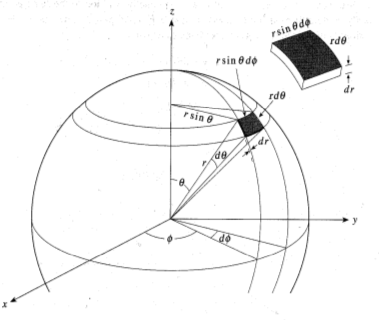
\includegraphics[scale=0.4]{ch1/image1}
	\captionof{figure}{ }
	\end{wrapfigure}
Avant toute chose, commençons par rappeler le système de coordonnées sphérique
\begin{equation}
\left\{\begin{array}{ll}
x &= r\sin\theta\cos\phi\\
y &= r\sin\theta\sin\phi\\
z &= r\cos\theta
\end{array}\right.
\end{equation}
Il convient de ne pas oublier le jacobien lors du changement de variable
\begin{equation}
d\vec{r} = dxdydz : (r\sin\theta d\phi)(rd\theta)dr = r^2\sin\theta drd\theta d\phi
\end{equation}

\subsection{Les harmoniques sphériques}
Le moment cinétique orbital $\vec{L}$ au carré s'écrit
\begin{equation}
\vec{L}^2 = \vec{L}.\vec L = L^2_x+L^2_y+L^2_z
\end{equation}
En coordonnée sphériques
\begin{equation}
\vec L^2 = -\hbar^2\left[\frac{1}{\sin\theta}\frac{\partial}{\partial \theta}\left(\sin\theta\frac{\partial}{
\partial \theta}\right)+\frac{1}{\sin^2\theta}\frac{\partial^2}{\partial\phi^2}\right]
\end{equation}
Les \textbf{harmoniques sphériques} sont par définition fonction propres de $\vec{L}^2$, mais aussi $L_z$\\

\cadre{\begin{equation}
\begin{array}{ll}
\vec{L}^2Y_{lm}(\theta,\phi) &= \hbar^2l(l+1)Y_{lm}(\theta,\phi)\\
L_z Y_{lm}(\theta,\phi) &= \hbar mY_{lm}(\theta,\phi)
\end{array}
\end{equation}
où $l=0,1,2,3,\dots$ et $m= l,l-1,l-2,\dots, -l$.}\ \\

Le choix de $m$ (pour \textit{magnétique}) prendra tout son sens lorsque l'on plongera le système dans un 
champ magnétique et que l'on perdra la symétrie sphérique par le fait qu'il existe une direction privilégiée. 
Comme ces deux observables ont des fonctions propres communes, elles doivent forcément commuter
\begin{equation}
[\vec{L}^2, L_z] = 0
\end{equation}
Pour nommer les orbitales, on donne un doux nom à chaque valeur de $l$\\

\cadre{$$l=0,1,2,3,4,5,6,7,\dots$$ $$s,p,d,f,h,i,k,\dots$$
où la lettre $j$ a volontairement été laissée sur le côté pour ne pas la confondre avec de $i$, ce qui 
pouvait facilement être le cas en utilisant des machines à écrire !}\ \\

Pour les retenir, un petit moyen mnémotechnique : \textit{"\textbf{S}olar \textbf{P}hysicists \textbf{D}on't
\textbf{F}ind \textbf{G}iraffes \textbf{H}idding \textbf{I}n \textbf{K}itchens}.\\

Les harmoniques sphériques sont définies pour $m \geq 0$ par 
\begin{center}
\textbf{INCLURE EQ SLIDE 4}
\end{center}
Dans le cas où $m$ est négatif, on trouve l'harmonique sphérique associée via : 
\begin{center}
\textbf{INCLURE EQ SLIDE 4}
\end{center}
Les harmoniques sphériques répondent aux relations d'orthonormalité, où il convient de ne pas oublier le 
facteur en $\theta$. Le prix à payer est bien évidemment celui de la normalisation :
\begin{center}
\textbf{INCLURE EQ SLIDE 4}
\end{center}

On peut définir des opérateurs de montée et de descente
\begin{equation}
L_+ \equiv L_x+iL_y,\qquad\qquad\qquad\qquad L_- \equiv L_x-iL_y
\end{equation}
Avec ceux-ci, il est possible de modifier la valeur de la projection du nombre quantique $l$, c'est-à-dire
$m_l$ (ou encore, $m$)
\begin{equation}
L_\pm Y_{lm}(\theta,\phi) = \hbar\sqrt{l(l+1)-m(m\pm 1)}Y_{lm\pm1}(\theta,\phi)
\end{equation}
Suivant cette définition, quelques harmoniques sphériques sont données au \textit{slide 5}.



\subsection{Les forces centrales}
Un potentiel central est un potentiel présentant une symétrie sphérique
\begin{equation}
V(\vec{r}) = V(r)
\end{equation}
où $r = |\vec r|$. Pour traiter ce potentiel de façon efficace, il convient d'écrire l'Hamiltonien 
\begin{equation}
H = -\frac{\hbar^2}{2m}\nabla^2+V(r)
\end{equation}
en coordonnées sphériques
\begin{equation}
H = -\frac{\hbar^2}{2m}\left[\frac{1}{r^2}\frac{\partial}{\partial r}\left(r^2\frac{\partial}{\partial r}\right)
+\frac{1}{r^2\sin\theta}\frac{\partial}{\partial \theta}\left(\sin\theta\frac{\partial}{\partial \theta}\right)
+ \frac{1}{r^2\sin^2\theta}\frac{\partial^2}{\partial \phi^2}\right] + V(r)
\end{equation}
En utilisant l'écriture sphérique de $\vec{L}^2$
\begin{equation}
\vec L^2 = -\hbar^2\left[\frac{1}{\sin\theta}\frac{\partial}{\partial \theta}\left(\sin\theta\frac{\partial}{
\partial \theta}\right)+\frac{1}{\sin^2\theta}\frac{\partial^2}{\partial\phi^2}\right]
\end{equation}
On peut écrire l'Hamiltonien sous une forme sphérique
\begin{equation}
H=-\frac{\hbar^2}{2m}\left[\frac{1}{r^2}\frac{\partial}{\partial r}\left(r^2\frac{\partial}{\partial r}\right)
-\frac{\vec L^2}{\hbar^2 r^2}\right] + V(r)
\end{equation}
Cet Hamiltonien vérifie les relations de commutation suivante
\begin{equation}
[H,\vec{L}^2] = [H,L_z] = [\vec{L}^2,L_z] = 0
\end{equation}
Il est possible de résoudre l'équation de Schrödinger par la méthode de séparation des variables, à l'aide
de nos harmoniques sphériques
\begin{equation}
\psi_{E,l,m}(r,\theta,\phi) = R_{E,l}(r)Y_{lm}(\theta,\phi)
\end{equation}
On peut alors obtenir l'équation radiale
\begin{equation}
\left\{-\frac{\hbar^2}{2m}\left[\frac{1}{r^2}\frac{d}{dr}\left(r^2\frac{d}{dr}\right) - \frac{l(l+1)}{r^2}\right]+
V(r)\right\}R_{E,l}(r) = ER_{E,l}(r)
\end{equation}
En effectuant le changement de variable $P_{E,l}(r) \equiv rR_{E,l}(r)$, on retrouve une équation de 
Schrödinger sous un format "classique"
\begin{equation}
\left[-\frac{\hbar^2}{2m}\frac{d^2}{dr^2}+\frac{\hbar^2l(l+1)}{2mr^2}+V(r)\right]P_{E,l}(r) = EP_{E,l}(r)
\end{equation}
On retiendra le comportement asymptotique suivant, pour $r\to0$ : $P_{E,l}(r) \sim r^{l+1}$.\\


La fonction factorisée $\psi_{E,l,m}(r,\theta,\phi) = R_{E,l}(r)Y_{lm}(\theta,\phi)$ respecte les règles 
d'inversion et de parité. On défini l'opération d'inversion (ou parité)
\begin{equation}
I\psi_{E,l,m}(\vec{r}) = I\psi_{E,l,m}(-\vec{r})
\end{equation}
Comme $I = I^\dagger$, ses valeurs propres sont réelles. Grâce à sa commutation avec l'Hamiltonien, on peut
écrire
\begin{equation}
[H,I]=0\Rightarrow I\psi_{E,l,m}(r)=\alpha\psi_{E,l,m}(r)
\end{equation}
Comme $I^2=E$, il en vient que $\alpha^2$ est forcément l'unité. Dès lors, $\alpha = \pm1$. Ceci revient à 
effectuer le changement de variable suivant (en cartésien et sphérique)
\begin{equation}
\left\{\begin{array}{ll}
x &\to -x\\
y &\to -y\\
z &\to -z
\end{array}\right. \qquad\qquad\qquad\left\{\begin{array}{ll}
r &\to -r\\
\theta &\to (\pi-\theta)\\
\phi &\to (\phi+\pi)
\end{array}\right. 
\end{equation}
Appliquons cet opérateur sur notre fonction factorisée :$I\psi_{E,l,m}(r,\theta,\phi) = I[R_{E,l}(r)Y_{lm}(\theta,
\phi)]$. Ceci donne
\begin{equation}
I\psi_{E,l,m}(r,\theta,\phi) = R_{E,l}(r)[IY_{lm}(\theta,\phi)] = (-1)^lR_{E,l}(r)Y_{lm}(\theta,\phi)
\end{equation}
où l'on voit apparaître la fonction factorisée. Nous avons ainsi défini l'effet de l'application de l'opérateur
parité sur la fonction d'onde \\

\cadre{
\begin{equation}
I\psi_{E,l,m}(r,\theta,\phi) = (-1)^l\psi_{E,l,m}(r,\theta,\phi)
\end{equation}}\ \\

Ainsi, $l$ pair implique $\alpha=+1$ et l'on parlera d'états \textbf{pairs}. A l'inverse, on parlera d'états
\textbf{impairs}.




\subsection{Problème à 2 corps: effet de masse}
Considérons deux particules en interaction
\begin{equation}
H = \frac{\vec p_1^2}{2m_1}+\frac{\vec p_2^2}{2m_2}+V(\vec r_1-\vec r_2)
\end{equation}
A l'aide du principe de correspondance $p\to -i\hbar\vec\nabla$ et $\vec{L}\to \vec{L}=-i\hbar(\vec{r}\times
\vec\nabla)$, on peut retrouver l'équation de Schrödinger
\begin{equation}
i\hbar\frac{\partial}{\partial t}\Psi(\vec{r}_1,\vec{r}_2, t) = \left[-\frac{\hbar^2}{2m_1}\nabla_1^2
-\frac{\hbar^2}{2m_2}\nabla_2^2+V(\vec r_1-\vec r_2)\right]\Psi(\vec{r}_1,\vec{r}_2, t)
\end{equation}
où $V$ ne dépend que de la coordonnée relative $\vec{r} =\vec{r_1}-\vec{r_2}$. Il est également pratique 
d'exprimer la coordonnée relative du centre de masse $\vec{R} = \frac{m_1\vec r_1+m_2\vec r_2}{m_1+m_2}$.
Effectuons alors le changement de coordonnées $(\vec{r_1},\vec{r_2})\to (\vec{r},\vec{R})$. Ceci peut se 
faire en définissant la masse totale et la masse réduite
\begin{equation}
M=m_1+m_2,\qquad\qquad\qquad \mu = \frac{m_1m_2}{m_1+m_2}
\end{equation}
En définissant le moment relatif $\vec{p}=\frac{m_2\vec p_1-m_1\vec p_2}{m_1+m_2}$ et le moment total $\vec{P}
= \vec{p_1}+\vec{p_2}$, nous avons que
\begin{equation}
\frac{\vec p_1^2}{2m_1}+\frac{\vec p_2^2}{2m_2} = \frac{\vec P^2}{2M}+\frac{\vec p^2}{2\mu}
\end{equation}
L'équation de Schrödinger devient
\begin{equation}
i\hbar\frac{\partial}{\partial t}\Psi(\vec R, \vec r, t) = \left[-\frac{\hbar^2}{2M}\nabla_R^2
-\frac{\hbar^2}{2\mu}\nabla_r^2+V(\vec r)\right]\Psi(\vec R, \vec r, t)
\end{equation}
où l'on voit cette fois-ci clairement apparaître la masse réduite $\mu$. Lorsque le potentiel $V$ est 
indépendant du temps $t$, il est possible d'effectuer le découplage du centre de masse et du mouvement 
relatif
\begin{equation}
\Psi(\vec R, \vec r, t) = \Phi(\vec{R})\psi(\vec{r})e^{-i(E_{CM}+E)t/\hbar}
\end{equation}
Ce découplage implique que l'on considère une particule libre de masse $M$ pour le centre de masse
\begin{equation}
-\frac{\hbar^2}{2M}\Delta_R^2\Phi(\vec{R}) = E_{CM}\Phi(\vec{R})
\end{equation}
Nous avons également à considérer une particule de masse $\mu$, cette fois-ci dans un potentiel $V(r)$
\begin{equation}
\left[-\frac{\hbar^2}{2\mu}\nabla_r^2+V(r)\right]\psi(\vec{r}) = E\psi(\vec{r})
\end{equation}
où nous retrouvons bien la masse réduite. Dans le contexte de l'atome d'hydrogène, celle-ci sera proche de la
masse de l'électron. \\

L'énergie totale à considérée est bien donnée par
\begin{equation}
E_{tot} = E_{CM}+E
\end{equation}


\subsection{Systèmes hydrogénoïdes – Potentiel de Coulomb}
Pour un système hydrogénoïde, nous devons utiliser l'équation décrivant le mouvement relatif
\begin{equation}
\left[-\frac{\hbar^2}{2\mu}\nabla_r^2+V(r)\right]\psi(\vec{r}) = E\psi(\vec{r})
\end{equation}
En utilisant comme potentiel le potentiel de \textsc{Coulomb} (potentiel central)
\begin{equation}
V(\vec{r}) = V(r) = -\dfrac{Ze^2}{4\pi\epsilon_0r}
\end{equation}
Celui-ci est le reflet d'un potentiel liant (négatif, ceci reflétant de \textsc{Coulomb} liant deux charges
opposées).

Cherchons les solutions en coordonnées sphérique $\psi_{E,l,m}(r,\theta,\phi) = R_{E,l}(r)Y_{lm}(\theta,\phi)$. 
L'équation radiale s'écrit
\begin{equation}
\left\{-\frac{\hbar^2}{2\mu}\left[\frac{1}{r^2}\frac{d}{dr}\left(r^2\frac{d}{dr}\right) - \frac{l(l+1)}{r^2}\right]+
V(r)\right\}R_{E,l}(r) = ER_{E,l}(r)
\end{equation}
où $r$ est la coordonnées relative et où ce n'est pas la masse de l'électron $m$ qui apparaît mais la masse
réduite $\mu$. C'est l'effet de masse qui apparaît lorsque les choses sont traitées correctement. Avec le 
changement de variable $P_{E,l}(r) \equiv rE_{E,l}(r)$ et en substituant , on trouve\\

\cadre{
\begin{equation}
\left[-\frac{\hbar^2}{2\mu}\frac{d^2}{dr^2}+\frac{\hbar^2l(l+1)}{2\mu r^2}-\frac{Ze^2}{4\pi\epsilon_0r}\right]P_{E,l}(r) = EP_{E,l}(r)
\end{equation}
\danger\ C'est bien la masse réduite $\mu$ qui apparaît ici.}\ \\

Cette équation permet de décrire les systèmes hydrogénoïdes, c'est-à-dire les systèmes atomiques à un seul
électron ($Z=1 : H, Z=2 : He^+, Z=91 :\  ^{91}U^{90+}, \dots$).\\


	\begin{wrapfigure}[14]{r}{4cm}
	\vspace{-5mm}
	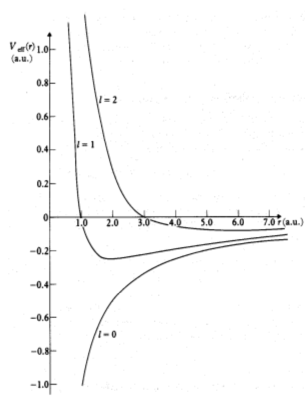
\includegraphics[scale=0.4]{ch1/image2}
	\captionof{figure}{ }
	\end{wrapfigure}
Pour retrouver une équation de Schrödinger "classique", on définit le \textit{potentiel effectif} $V_{eff}^{(l)}$
\begin{equation}
V_{eff}^{(l)} = -\frac{Ze^2}{4\pi\epsilon_0r}+\dfrac{l(l+1)\hbar^2}{2\mu r^2}
\end{equation}
Le second terme du membre de droite est le \textit{potentiel centrifuge} qui, contrairement au potentiel
de \textsc{Coulomb}, est antiliant (signe positif). Le potentiel effectif est déterminé par la valeur de
$l$ : une valeur nulle de $l$ donne le potentiel coulombien.\\

Cependant, dès que $l\neq 0$, une nouvelle contribution à petite distance apparaît. Elle relève l'existence d'un
potentiel centrifuge qui fait que l'on a une barrière coulombienne que l'on ne retrouve pas pour $l=0$. Ceci
explique le comportement différent pour un électron $s$ ou $p$, le potentiel étant totalement différent.


\newpage
\subsection{Solution pour les états liés}
La solution de l'équation ci-dessus pour des états liés est donnée par 
\begin{equation}
E_n = -\frac{1}{2n^2}\left(\frac{Ze^2}{4\pi\epsilon_0}\right)^2\frac{\mu}{\hbar^2}=-\frac{e^2}{(4\pi\epsilon_0)
a_0}\left(\frac{\mu}{m}\right)\frac{Z^2}{2n^2}
\end{equation}
où $a_0=\frac{(4\pi\epsilon_0)\hbar^2}{me_2}$ est le rayon de \textsc{Bohr}.\\

	\begin{wrapfigure}[23]{l}{8.5cm}
	\vspace{-5mm}
	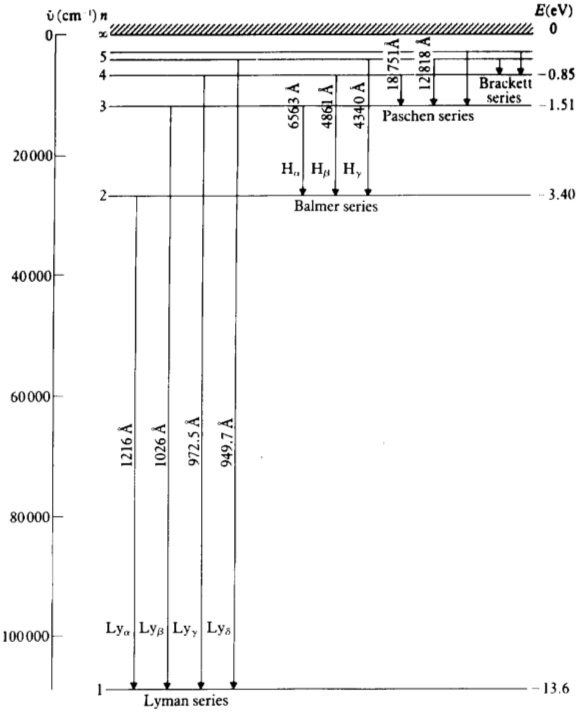
\includegraphics[scale=0.4]{ch1/image3}
	\captionof{figure}{ }
	\end{wrapfigure}
	
	Ci-contre, la représentation de la solution pour les états liés dans le cadre de l'atome d'hydrogène
	($Z=1, \mu=m$). La première chose que l'on peut constater est la présence de transition dans quasi toutes
	les classes, tout dépend de la transition regardées. On retrouve les raies de \textsc{Lyman} (transitions
	vers $n=1$), les raies de \textsc{Balmer} (transitions vers $n=2$), les raies de \textsc{Paschen}
	(transitions vers $n=3$) mais également les raies de \textsc{Brackett} (transitions vers $n=4$).\\
	
	Pour l'état $n=2$, on retrouve les états $2s_0, 2p_{+1}$ et $2p_{-1}$ qui sont tous caractérisés par
	une énergie $E_2$ donnée par la solution ci-dessus. Le niveau fondamental (énergie de 13.6 eV) n'est 
	autre que l'état $1s$. On note souvent les énergie en $cm^{-1}$, d'où l'échelle verticale. Si on regarde
	la différence entre $n=2$ et $n=1$, elle vaut à peu près $100'000$ cm$^{-1}$. Il s'agit du \textbf{
	nombre d'onde} défini comme l'inverse de la longueur d'onde. Plusieurs écritures sont possibles
	\begin{equation}
	\frac{1}{\lambda}\equiv \bar\lambda = \sigma = \bar\nu
	\end{equation}
	La longueur d'onde est l'inverse de cette "distance" et on retrouve bien la valeur de 1216 Angström. 
	Il existe une relation donnant la fréquence en fonction de la différence de l'inverse de deux nombres 
	entiers multipliée par une certaine constante afin que ce soit correction dimensionnement
	\begin{equation}
	\nu = R_\infty\left(\frac{1}{n_1^2}-\frac{1}{n_2^2}\right)\qquad\text{où }\quad R_\infty = \frac{m}{
	4\pi\hbar^3}\left(\frac{e^2}{4\pi\epsilon_0}\right)^2
	\end{equation}
	

\subsection{Système d'unités atomiques}
Le système d'unité atomique est un système horrible ou tout vaut 1. Avant de l'énoncer, rappelons la 
définition du rayon de \textsc{Bohr}
\begin{equation}
a_0=\frac{(4\pi\epsilon_0)\hbar^2}{me_2} = 5.29\times 10^{-11}\text{ m}
\end{equation}
On dira que $a_0$ = 1 u.a. de longueur. Si on veut savoir, ce que ça vaut, il faudra faire les bonnes
substitution dans la formule de $a_0$ sachant que
$m=m_e$ = 1 u.a. de masse, $e$ = 1 u.a. de charge, $\hbar$ = 1 u.a. de moment angulaire et $4\pi\epsilon_0$ =
1 u.a.  de permittivité du vide. Ce choix d'unité est fait pour déterminer avec intelligence l'énergie. Si on 
évalue l'énergie $E_n$ ci-dessus avec ces unités, presque tout va se simplifier.\\

Sachant que une unité atomique d'énergie est donnée par $E_h = e^2/(4\pi\epsilon_0 a_0)$, il est vient que
$E_n \approx -\frac{Z^2}{2n^2}E_h$. Pour $Z=1$, on trouve $E_{n=1} \approx -1/2 E_h$. Il est possible de 
retrouver la valeur sachant que $1 E_h$ (un hartree) vaut 27.2 eV.\\

Ce système simplifie également les vitesses
\begin{equation}
v_0 = \frac{e^2}{(4\pi\epsilon_0)\hbar}\equiv \alpha c = 1 \text{ u.a. de vitesse}
\end{equation}
Comme $\alpha \approx 1/137$, on en déduit que $c\approx 137$ u.a. de vitesse.\\


\subsection{Solutions pour les états liés}
Compte tenu de ce système d'unité, on peut alors ré-écrire la solution pour les états liés d'énergie $E_n$
\begin{equation}
E_n = -\frac{e^2}{(4\pi\epsilon_0)a_\mu}\frac{Z^2}{2n^2}=-\dfrac{Z^2}{2n^2}\left(\frac{\mu}{m}\right)\text{ u.a.}
\end{equation}
\begin{center}
\textbf{INCLURE QUELQUES EX SLIDE 18}
\end{center}
où l'on possède une loi d'échelle reliant $\rho$ à $r$.



\subsubsection{Densités radiales}
Le \textit{slide 19} donne des exemples de densité radiale, justifiant la structure en couche des 
électrons et orbitales dans les systèmes polyélectroniques. On remarque que lorsqu'il y a deux nœuds 
radiaux, on les retrouve dans la structure en densité (qui s'annule la où la fonction radiale s'annule). Elles
sont forcément positives car elle détermineront les densités de probabilités.\\

On remarque que $2s$ s'éteint de façon exponentielle, sans nœud. La grande différence entre l'orbitale $s$ et
les autres est qu'elle est non-nulle en $r=0$ (car pas de potentiel centrifuge).

\begin{center}
\textbf{INCLURE QUELQUES EX SLIDE 19}
\end{center}

\newpage
\section{Spectre de l’atome d’hydrogène}

\subsection{Série de Balmer}
	\begin{wrapfigure}[12]{l}{8cm}
	\vspace{-5mm}
	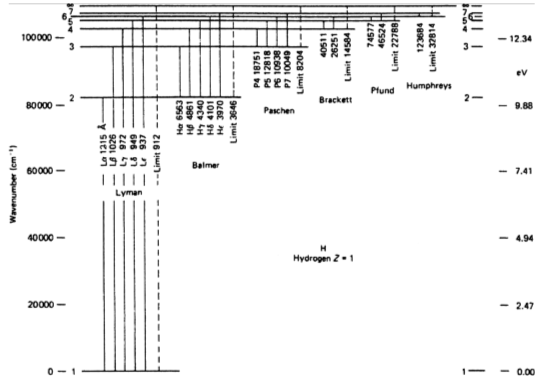
\includegraphics[scale=0.4]{ch1/image4}
	\captionof{figure}{ }
	\end{wrapfigure}
\textsc{Balmer} a observé une série de raie qui convergent vers une certaine limite, l'ionisation. Ainsi, la
raie qui a la plus proche longueur d'onde se rapproche de l'ionisation (il s'agit donc de la plus grande 
transition de \textsc{Balmer} en nombre de cm$^{-1}$ sur le spectre vu précédemment). Le spectre (version 
nombre d'onde $1/\lambda$) peut s'obtenir via
\begin{equation}
\tilde{\nu} = \tilde{R}\left(\frac{1}{n_1^2}-\frac{1}{n_2^2}\right)
\end{equation}
où $\tilde{R}_H = 109\ 677.58\ \text{cm}^{-1}$.\\

En fixant $n_1$ ($< n_1$) et en faisant flotter $n_2$ on peut retrouver les séries de
\begin{multicols}{2}
\begin{description}
\item[Lyman] $n_1=1$, UV
\item[Balmer] $n_1=2$, visible
\item[Paschen] $n_1=3$, IR
\item[Brackett] $n_1=4$, IR (lointain)
\item[Pfund] $n_1=5$, IR (très lointain)
\item[Hymphreys] $n_1=6$, IR (presque radio)
\end{description}
\end{multicols}


\subsection{Règle de Laporte et nomenclature}
	\begin{wrapfigure}[13]{r}{5.5cm}
	\vspace{-5mm}
	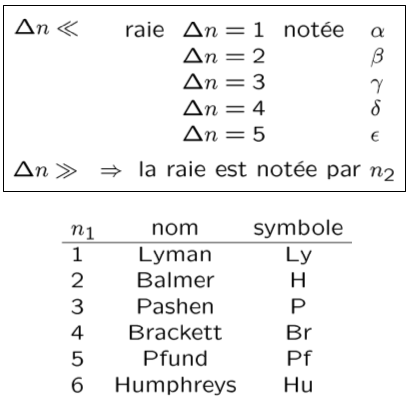
\includegraphics[scale=0.4]{ch1/image5}
	\captionof{figure}{ }
	\end{wrapfigure}
Il s'agit d'une représentation proposée par \textsc{Grotrian}. Celle-ci se base sur une représentation des
ensemble des niveaux avec les transitions permises et les règles de sélection. La règle de \textsc{Laporte} 
(Règle de sélection ($E1$) : $\Delta l = \pm 1$). sera approfondie au chapitre 3. \\

Le nombre d'onde s'exprime
\begin{equation}
\bar \nu = \frac{1}{\lambda} = \frac{1}{hc}(E_{n_1}-E_{n_2}) = \bar R_H\left(\frac{1}{n^2_1}-\frac{1}{n^2_2}
\right)
\end{equation}
On définit également
\begin{equation}
\bar{R}_H = \frac{\mu}{m_e}\bar{R}_\infty = \left(\frac{M_H}{M_H+m_e}\right)\bar{R}_\infty
\end{equation}
où $\bar{R}_H = 109677.581$ cm$^{-1}$ et $\bar{R}_\infty = 109737.31$ cm$^{-1}$.



\subsection{Effet de masse : Hydrogène et Deutérium}
Dans le spectre d'émission de l'hydrogène, on remarque que l'on a une raie très proche aux alentours de la
première raie (la plus à gauche)\footnote{Juste à côté de $H\alpha$ (voir nomenclature), on devine la présence
d'une autre raie : c'est celle du deutérium.}. Calculons l'émission de $H\alpha$
\begin{equation}
\bar\nu = \frac{1}{\lambda}= \bar{R}_H\left(\frac{1}{4}-\frac{1}{9}\right) = 15237\ \text{cm}^{-1}
\end{equation}

\newpage
	\begin{wrapfigure}[14]{l}{6cm}
	%\vspace{-5mm}
	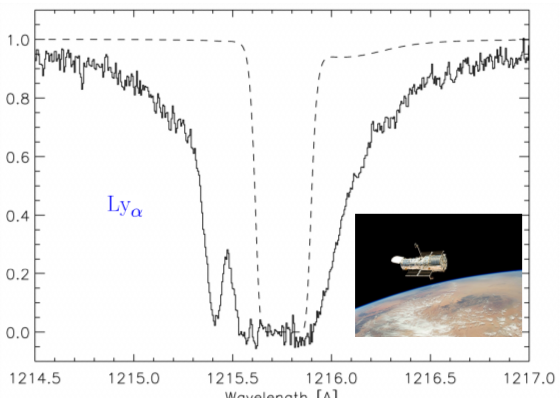
\includegraphics[scale=0.3]{ch1/image6}
	\captionof{figure}{On remarque un \textit{pic de deutérium} sur la \textsc{Lyman}$\alpha$. Elle se 
	situe dans l'UV (longueur d'onde plus petite que celle de l'hydrogène).}
	\end{wrapfigure}
Sachant que\footnote{Revoir le sens de $R$. D'où ça sort?} pour le deutérium $R_D = \frac{\mu_D}{\mu_H}R_H$ 
et connaissant $M_H$ et $M_D$, on peut évaluer le rapport des deux
\begin{equation}
\frac{\mu_D}{\mu_H} = \left(\frac{M_H+m_e}{M_Hm_e}\right)\left(\frac{M_Dm_e}{M_D+m_e}\right)=1.00027
\end{equation}
Il y a émission $H\alpha$ dans le deutérium à 15233 cm$^{-1}$. Il faut donc une très bonne résolution pour
pouvoir l'observer : il s'agit d'un effet plus fin que la structure fine. On définit le \textit{rapport 
d'abondances cosmiques}
\begin{equation}
\frac{[D]}{[H]}=2\times 10^{-5}
\end{equation}
Ceci signifie que les raies de l'hydrogène seront souvent \textit{optically thick} si celle de $D$ sont 
observables.

\section{Spectre des systèmes hydrogénoïdes}
\subsection{Loi d'échelle}
	\begin{wrapfigure}[14]{r}{6cm}
	\vspace{-8mm}
	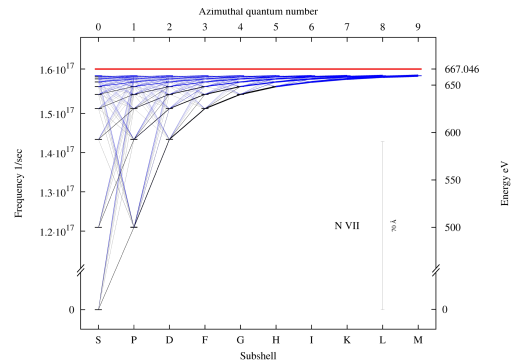
\includegraphics[scale=0.35]{ch1/image7}
	\captionof{figure}{ }
	\end{wrapfigure}
L'azote sept (en lettre grecques, $N\ VII$ ou $N^{6+}$ ($Z=7$)) est le septième spectre de l'azote. Il
est hydrogénoïde car bien qu'il possède sept protons, il n'a qu'un seul électron. On remarque que 
\begin{equation}
\begin{array}{lll}
E_n &=\DS -\frac{1}{2n^2}\left(\frac{Ze^2}{4\pi\epsilon_0}\right)^2\frac{m_e}{\hbar^2}\qquad \ &\propto
 Z^2\vspace{2mm}\\
I_P &=\DS \frac{1}{2}\frac{m_e}{\hbar^2}\left(\frac{Ze^2}{4\pi\epsilon_0}\right)^2 &=13.6\ Z^2\ \text{eV}
\end{array}
\end{equation}
On voit ainsi un effet liant de la charge sur le spectre (la proportionnalité en $Z^2$). Plus $Z$ augmente, 
plus $\bar R_M$ tend vers $\bar R_\infty = 109\ 737.32$. En effet, plus $Z$ augmente plus les niveaux sont
écartés mais plus la longueur d'onde diminue (évolue en $Z^{-2}$). Cette augmentation de $Z$ causant une 
diminution de $\lambda$ et une augmentation de $\bar R_M$ implique que le seul électron restant est 
"de plus en plus léger". La correction de masse est donc d'autant plus grande que le noyau est léger.\\

Il faut également prendre en compte les effets relativiste. Connaissant la vitesse de l'électron dans 
la première orbite de \textsc{Bohr}, on peut établir le rapport suivant
\begin{equation}
\frac{v}{c} = \alpha Z \approx \frac{Z}{137}
\end{equation}
Si $Z$ est faible, on peut négliger les effets relativiste. Par contre, si $Z$ est de l'ordre de 100, cela
signifie que la vitesse de l'électron est plus élevée : il va falloir prendre en compte les effets 
relativites. La vitesse de l'électron est ainsi d'autant plus grande que le nombre de proton est élevé. 
Passé un certain nombre, il faudra passer en relativiste et utiliser \textsc{Dirac} et non plus
\textsc{Schrödinger}\footnote{Pour un $Z$ grand, même dans un système hydrogénoïde, il faudra tenir compte
des effets relativiste. Notons qu'il n'y a pas de contradiction pour $Z>137$ (c'est bien possible) . Il 
faut en effet se rappeler que la vitesse de l'électron est estimée d'un modèle non-relativite.}.



















\section{Le spin électronique}
\section{Effets relativistes et structure fine}